
%(BEGIN_QUESTION)
% Copyright 2012, Tony R. Kuphaldt, released under the Creative Commons Attribution License (v 1.0)
% This means you may do almost anything with this work of mine, so long as you give me proper credit

Suppose the diaphragm actuator on an air-to-open pneumatic valve has a bench-set range of 6 to 30 PSI, a diaphragm diameter of 13 inches, and a 1-inch stroke length.  Calculate the amount of work done by the actuator in moving the valve from fully-closed to fully-open.  Also, calculate the amount of {\it seat load} (i.e. the amount of force exerted by the spring on the plug of the valve to keep it fully seated when there is zero pressure applied to the diaphragm): 

\vskip 10pt

Work = \underbar{\hskip 50pt} ft-lb

\vskip 10pt

Seat load = \underbar{\hskip 50pt} lb

\underbar{file i01107}
%(END_QUESTION)





%(BEGIN_ANSWER)

The work done by the valve actuator must be calculated as an integral, because the amount of force changes with displacement.  The shaded area in this graph represents the work done in lifting the valve stem 1 inch ($1 \over 12$ foot) with the 6-30 PSI actuating pressure acting upon a 13 inch circular diaphragm:

$$\includegraphics[width=15.5cm]{i01107x01.eps}$$

\vskip 10pt

The seat load is simply the amount of force exerted by the plug on the seat when there is no pressure applied to the actuator diaphragm.  This will be the exact same force required of the actuator to begin moving the plug off the seat, equal to 6 PSI applied to the 13 inch diameter diaphragm.  Thus, the seating force is \underbar{\bf 796.4} pounds.

%(END_ANSWER)





%(BEGIN_NOTES)

{\bf This question is intended for exams only and not worksheets!}.

%(END_NOTES)


